
\documentclass[11pt,a4paper]{article}

\usepackage[utf8]{inputenc}
\usepackage[T1]{fontenc}
\usepackage[spanish]{babel}

\usepackage{tgpagella}
\usepackage{geometry}
\usepackage{graphicx}
\usepackage{xcolor}
\usepackage{titlesec}
\usepackage{fancyhdr}
\usepackage[parfill]{parskip}
\usepackage[expansion=false]{microtype}
\usepackage{hyperref}
\usepackage{setspace}
\usepackage{needspace}

\geometry{top=3.0cm,bottom=3.0cm,left=3.5cm,right=3.5cm}

\setlength{\parskip}{0.65em}
\setlength{\parindent}{0em}

\definecolor{azulai}{RGB}{30,80,140}
\definecolor{doradoai}{RGB}{140,90,0}
\definecolor{grisai}{RGB}{70,70,70}

\titleformat{\section}
{\Large\bfseries\color{azulai}}
{}{0em}{}
[{\color{azulai}\titlerule[0.5pt]}]

\titlespacing*{\section}{0pt}{1.8em}{0.8em}

\titleformat{\subsection}
{\large\bfseries\color{doradoai}}
{}{0em}{}

\titlespacing*{\subsection}{0pt}{1.2em}{0.4em}

\pagestyle{fancy}
\fancyhf{}

\rhead{\textcolor{grisai}{\small Amaya Beatriz — Arquitectura Interna}}
\lhead{\textcolor{grisai}{\small Carta Natal Base}}

\cfoot{\textcolor{grisai}{\small\thepage}}

\renewcommand{\headrulewidth}{0.3pt}

\hypersetup{
colorlinks=true,
linkcolor=azulai,
urlcolor=azulai
}

\setstretch{1.4}

\begin{document}

% ── PORTADA ──────────────────────────────────────────────────────────────

\begin{titlepage}

\centering

\vspace*{1.5cm}

{\Huge\bfseries\color{azulai} Carta Natal Base}\\[0.5cm]

{\large\color{grisai} Arquitectura Interna}\\[0.4cm]

{\small\itshape\color{grisai}
Un método para sostener cuerpo, energía y vida con coherencia
}\\[2cm]

{\huge\color{doradoai} Amaya Beatriz}\\[1.5cm]

{\Large 30/10/1976 \quad 22:10}\\[0.3cm]

{\Large Zaragoza, España}\\[0.3cm]

{\normalsize
Lat: 41.6916° \quad
Lon: -0.9101° \quad
UTC+01:00
}\\[0.5cm]

{\normalsize
Ascendente: Cáncer 16°08'
}\\[2.5cm]

\vfill

{\small Generado el 19/05/2026}

\end{titlepage}


% ── INTRODUCCIÓN ─────────────────────────────────────────────────────────────

\section*{Introducción}

Esta carta natal base no busca definir quién eres.

La astrología se utiliza aquí como lenguaje de observación:
una forma de mirar cómo se organiza tu energía,
qué registros aparecen con más facilidad
y qué dinámicas pueden influir en tu manera de vivir, sostenerte y relacionarte con el entorno.

No se trata de una lectura predictiva ni de una identidad fija.
Es un mapa inicial de orientación.

Las siguientes páginas muestran únicamente las capas principales de la carta:
los ejes más visibles,
la distribución general de la energía
y algunos patrones básicos desde los que sueles moverte.

\vspace{0.4cm}

\newpage


% ── RUEDA ────────────────────────────────────────────────────────────────

\section{Carta Natal}

\begin{center}
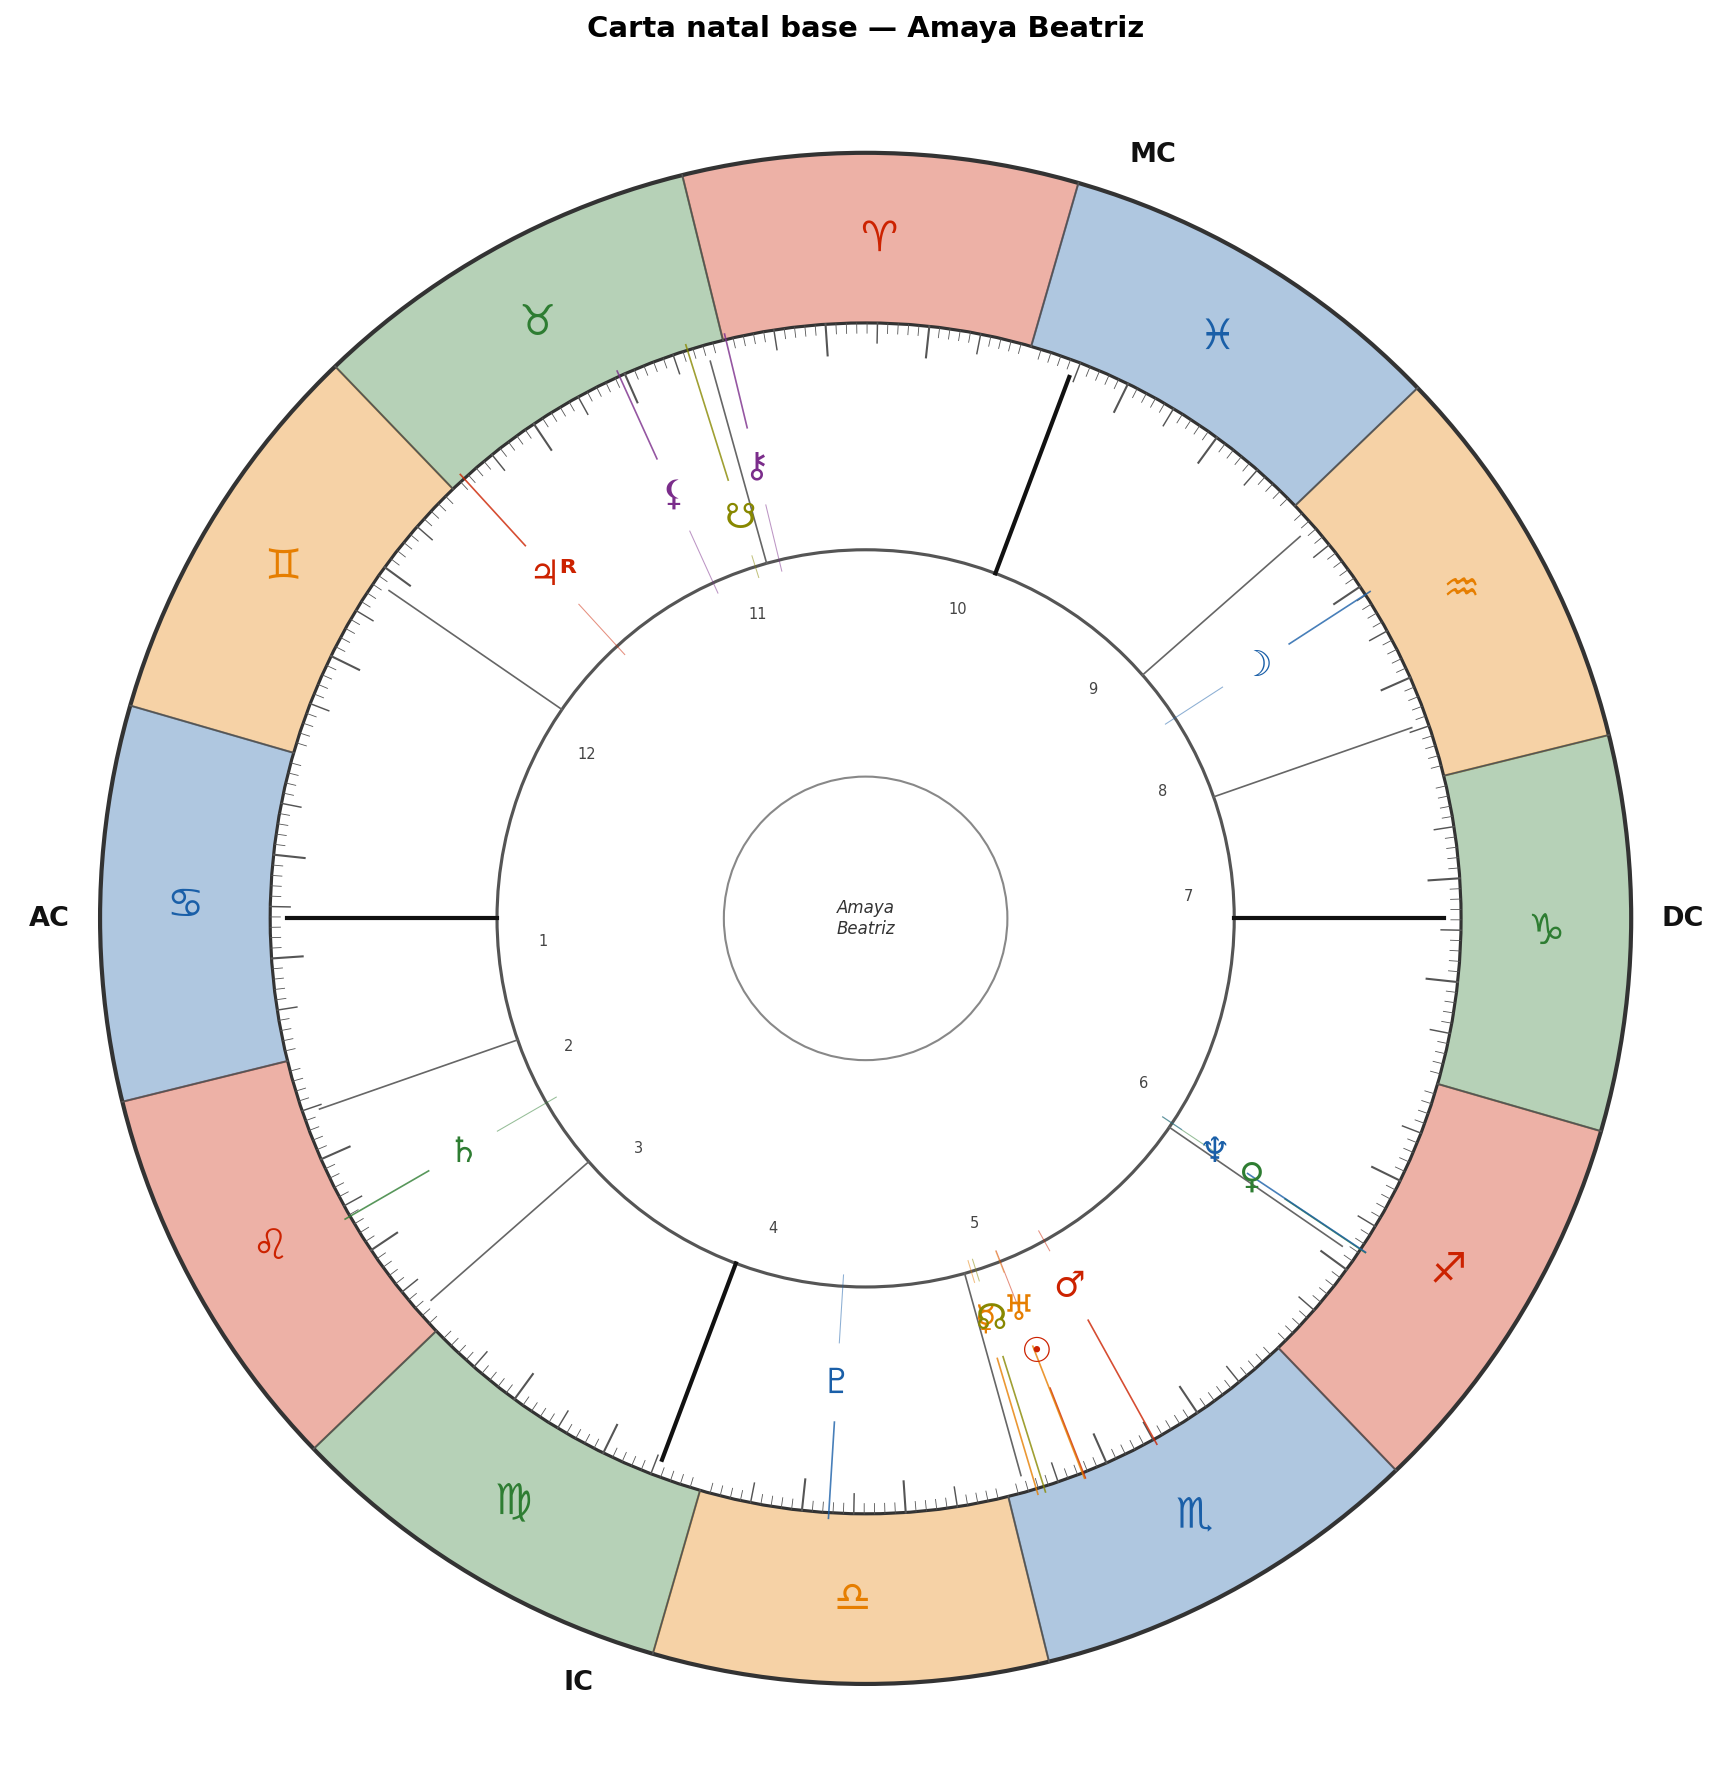
\includegraphics[width=0.8\textwidth]{Amaya_Beatriz_carta_base_rueda.png}
\end{center}

\vspace{0.8cm}

% ── POSICIONES PRINCIPALES ───────────────────────────────────────────────

\section{Posiciones principales}

\begin{center}

Sol en Escorpio — Casa 5\\
Luna en Acuario — Casa 8\\
Ascendente Cáncer\\
Medio Cielo en Piscis

\end{center}

\vspace{0.5cm}

{\small\itshape
La lectura ampliada desarrolla el mapa completo de posiciones,
aspectos y configuraciones de la carta.
}

\vspace{0.8cm}
\Needspace{5\baselineskip}

% ── VISIÓN GENERAL ───────────────────────────────────────────────────────

\section{Visión general}

Tu carta muestra esta distribución de elementos: Fuego 3.5, Tierra 1, Aire 4, Agua 8. El elemento más presente es Agua (sensibilidad, percepción emocional y conexión con el entorno). Esto señala un registro que suele aparecer con facilidad en tu forma de funcionar. El elemento menos presente es Tierra (estabilidad, concreción y contacto con lo práctico). No significa ausencia, sino una cualidad que puede necesitar más atención consciente. Predomina la modalidad fija, asociada a la constancia, la continuidad y la capacidad de sostener lo importante. Tu Medio Cielo en Piscis orienta tu presencia pública hacia la sensibilidad, imaginación y capacidad de adaptación.

\vspace{0.8cm}
\Needspace{5\baselineskip}

% ── LOS TRES PILARES ────────────────────────────────────────────────────

\section{Los tres pilares}

\subsection{Sol en Escorpio}

Con el Sol en Escorpio, suele haber necesidad de profundidad, implicación real e intensidad emocional. No te resulta fácil permanecer mucho tiempo en situaciones que sientes vacías o superficiales. Cuando algo te importa de verdad, normalmente tiendes a implicarte profundamente. Con el Sol en Casa 5, la creatividad, la expresión personal y la necesidad de disfrutar lo que haces suelen ocupar un lugar importante en tu vida. Necesitas sentir que puedes crear, compartir o expresar algo propio. Cuando hay espacio para la autenticidad y el disfrute, normalmente sueles sentirte más vital.

\vspace{0.8cm}
\Needspace{5\baselineskip}

\subsection{Luna en Acuario}

Con la Luna en Acuario, necesitas cierta libertad emocional y espacio propio para sentirte bien. Cuando las emociones son demasiado intensas o invasivas, puedes necesitar tomar distancia para entender lo que te ocurre. Los vínculos donde hay respeto por la individualidad suelen ser especialmente importantes para ti. Con la Luna en Casa 8, las emociones suelen vivirse con bastante intensidad aunque no siempre se expresen fácilmente. Los vínculos profundos y las experiencias importantes tienden a afectarte más de lo que otras personas perciben desde fuera.

\vspace{0.8cm}
\Needspace{5\baselineskip}

\subsection{Ascendente Cáncer}

Con Ascendente en Cáncer, normalmente te muestras de forma receptiva, sensible y bastante atenta al entorno. Sueles observar primero cómo es el ambiente antes de abrirte del todo. Las demás personas pueden percibir cierta suavidad o reserva en el primer contacto.

\vspace{0.8cm}
\Needspace{5\baselineskip}

% ── CIERRE ───────────────────────────────────────────────────────────────

\section{Cierre}

Esta carta no busca definirte ni darte una identidad fija.

La astrología se utiliza aquí como lenguaje de observación:
una forma de mirar tendencias, ritmos y maneras de relacionarte con la vida.

La lectura ampliada desarrolla con más profundidad:
los vínculos,
la regulación emocional,
los patrones repetitivos,
la dirección de crecimiento,
las tensiones internas
y las configuraciones principales de la carta.

La lectura completa no busca darte más información.
Busca ayudarte a entender cómo sostener tu vida sin romperte por dentro.

\vspace{1cm}

\begin{center}

{\small\itshape\color{grisai}
Arquitectura Interna
}

\end{center}

\end{document}
